Ada beberapa model algoritma yang sudah disediakan openCV untuk melakukan pengenalan wajah, diantaranya adalah
Eigenface, Fisherfaces, dan \emph{Local binary Pattern Histogram}(LBPH). Berikut penjelasan untuk perbedaan dari ketiga model algoritma yang disediakan olen openCV.
\section{Eigenface}

Eigenface adalah salah satu algoritma pengenalan wajah yang berdasarkan pada Principle Component Analysis (PCA) yang dikembangkan di MIT.
Algoritma EigenFace secara keseluruhan cukup sederhana, Training Image direpresentasikan dalam sebuah vektor flat (gabungan vektor) dan digabung
bersama-sama menjadi sebuah matriks tunggal. Eigen Vector kemudian diekstraksi dan disimpan dalam file temporary atau database. Training image
kemudian diproyeksikan dalam feature space yang di namai face space yang ditentukan oleh eigen vektor(Mukti, 2008).\footnote{Alam, R.G guntur, dkk.
\emph{MPLEMENTASI ALGORITMA EIGENFACE UNTUK FACE RECOGNITION PADA OBJECK FOTO ID CARD}.Telematik : Vol 7, No 2, April 2015.}
%http://repository.unib.ac.id/18865/1/4.%20IMPLEMENTASI%20ALGORITMA%20EIGENFACE%20UNTUK%20FACE.pdf

Principal Component Analysis (PCA) atau disebut juga transformasi KarhunenLoeve adalah tekhnik yang digunakan untuk menyederhanakan suatu data, dengan cara mentransormasi linear sehingga terbentuk
system koordinat baru dengan variansi maksimum. PCA dapat digunakan untuk mereduksi dimensi suatu data tanpa mengurangi karakteristik data tersebut secara signifikan (Cahyadi, 2007: 93)
\footnote{Firliana, Lina, dkk.\emph{Implementasi Principal Component Analysis (PCA) Untuk Pengenalan Wajah Manusia}. Universitas Nusantara}\\

Berikut proses langkah-langkah pengenalan wajah menggunakan model algoritma Eigenface.
\begin{enumerate}[1. ]
    \item Penyusunan flat vektor matriks
    \item Mengambil nilai tengah dari kumpulan matriks
    \item Menghitung selisih antara nilai matriks \emph{training image} dengan nilai tengah
    \item Menghitung nilai matriks kovarian
    \item Menghitung nilai \emph{eigenvalue} dan \emph{eigenvector}
    \item Menghitung nilai \emph{eigenface}
    \item Proses indentifikasi wajah 
\end{enumerate}

\section{Local Binary Pattern Histogram(LBPH)}
Local Binary Patter(LBP) adalah salah satu dari metode yang  terkenal dalam mengenali sebuah objek. Dalam hal ini, cara yang digunakan adalah membedakan objek dengan background. 
Local Binary Patter Histogram(LBPH) adalah sebuah kombinasi algoritma antara LBP dengan Histogram of Oriented Gradients(HOG)

\newpage
\section{Fisherfaces}
Algoritma Fisherface ini merupakan gabungan dari metode Principal Component Analys (PCA) dengan Fisher’s Linear Discriminant (FLD). FLD merupakan salah satu contoh metode class specific, 
karena prinsip dasar metode ini berusaha untuk membentuk jarak (scatter) antar kelas dan intra kelas sehingga dapat menghasilkan klasifikasi yang lebih baik, dan mereduksi dimensi yang didapat dari perhitungan PCA. 
Semakin besar rasio antar kelas, vector ciri yang dihasilkan semakin tidak sensitive terhadap perubahan ekspresi maupun perubahan pencahayaan, sehingga dapat menghasilkan klasifikasi yang lebih baik. 
\footnote{Amalia, Nurul. Perbandingan Algoritma Fisherface dan Algoritma Local Binary Pattern Untuk Pengenalan Wajah. Universitas Budi Darma, Medan}
\begin{figure}[h!]
    \centering
    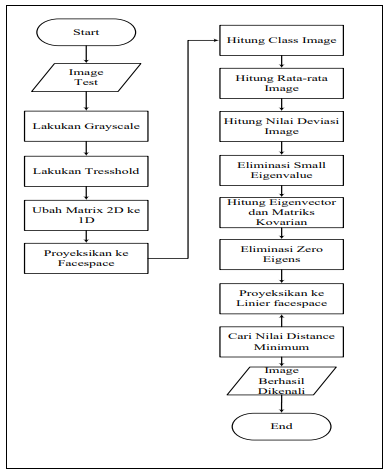
\includegraphics[width=0.7\linewidth]{images/algoritma_fisherface.PNG}
    \caption{Proses algoritma fisherface}
\end{figure}